% ============================================================
% Question Bank: ch05-06 Graphing Solutions to Inequalities on a Number Line
% Topic Title: Graphing Solutions to Inequalities on a Number Line
% CCSS: 7.EE.B.4b
% Questions: 27 (15 MC + 6 SA + 6 Graphical)
% ============================================================

% --- Multiple Choice Questions (15) ---

\begin{practiceQuestion}{5-6-q01}{mc}
\begin{questionText}
What type of circle is used to graph $x \leq 5$ on a number line?
\end{questionText}
\choiceA{Open circle at $5$}
\choiceB{Closed circle at $5$}
\choiceC{Open circle at $0$}
\choiceD{Closed circle at $0$}
\correctAnswer{B}
\explanation{$x \leq 5$ uses a closed circle because $5$ is included (less than \textbf{or equal to}).}
\end{practiceQuestion}

\begin{practiceQuestion}{5-6-q02}{mc}
\begin{questionText}
Which graph represents $x > -3$?
\end{questionText}
\choiceA{Closed circle at $-3$, shade right}
\choiceB{Open circle at $-3$, shade left}
\choiceC{Open circle at $-3$, shade right}
\choiceD{Closed circle at $-3$, shade left}
\correctAnswer{C}
\explanation{$x > -3$: open circle (does not include $-3$) and shade right (values greater than $-3$).}
\end{practiceQuestion}

\begin{practiceQuestion}{5-6-q03}{mc}
\begin{questionText}
Solve $2x + 3 \leq 15$ and choose the correct graph description.
\end{questionText}
\choiceA{Open circle at $6$, shade left}
\choiceB{Closed circle at $6$, shade left}
\choiceC{Closed circle at $6$, shade right}
\choiceD{Open circle at $9$, shade left}
\correctAnswer{B}
\explanation{Subtract $3$: $2x \leq 12$. Divide by $2$: $x \leq 6$. Closed circle at $6$ (includes $6$), shade left.}
\end{practiceQuestion}

\begin{practiceQuestion}{5-6-q04}{mc}
\begin{questionText}
Solve $4n - 8 > 12$ and describe the graph.
\end{questionText}
\choiceA{Open circle at $5$, shade right}
\choiceB{Closed circle at $5$, shade right}
\choiceC{Open circle at $1$, shade right}
\choiceD{Open circle at $5$, shade left}
\correctAnswer{A}
\explanation{Add $8$: $4n > 20$. Divide by $4$: $n > 5$. Open circle at $5$, shade right.}
\end{practiceQuestion}

\begin{practiceQuestion}{5-6-q05}{mc}
\begin{questionText}
Which inequality is shown by an open circle at $-4$ with shading to the left?
\end{questionText}
\choiceA{$x > -4$}
\choiceB{$x \leq -4$}
\choiceC{$x < -4$}
\choiceD{$x \geq -4$}
\correctAnswer{C}
\explanation{Open circle means $-4$ is not included, shading left means less than: $x < -4$.}
\end{practiceQuestion}

\begin{practiceQuestion}{5-6-q06}{mc}
\begin{questionText}
Solve $-3x \leq 15$ and describe the graph.
\end{questionText}
\choiceA{Closed circle at $-5$, shade left}
\choiceB{Closed circle at $5$, shade left}
\choiceC{Closed circle at $-5$, shade right}
\choiceD{Open circle at $-5$, shade right}
\correctAnswer{C}
\explanation{Divide by $-3$ and flip: $x \geq -5$. Closed circle at $-5$, shade right.}
\end{practiceQuestion}

\begin{practiceQuestion}{5-6-q07}{mc}
\begin{questionText}
The graph of an inequality has a closed circle at $8$ and is shaded to the left. Which inequality matches?
\end{questionText}
\choiceA{$x < 8$}
\choiceB{$x > 8$}
\choiceC{$x \leq 8$}
\choiceD{$x \geq 8$}
\correctAnswer{C}
\explanation{Closed circle means $8$ is included, shading left means less than or equal to: $x \leq 8$.}
\end{practiceQuestion}

\begin{practiceQuestion}{5-6-q08}{mc}
\begin{questionText}
Solve $5x + 2 \leq 27$ and describe the graph.
\end{questionText}
\choiceA{Open circle at $5$, shade left}
\choiceB{Closed circle at $5$, shade left}
\choiceC{Closed circle at $5$, shade right}
\choiceD{Closed circle at $25$, shade left}
\correctAnswer{B}
\explanation{Subtract $2$: $5x \leq 25$. Divide by $5$: $x \leq 5$. Closed circle at $5$, shade left.}
\end{practiceQuestion}

\begin{practiceQuestion}{5-6-q09}{mc}
\begin{questionText}
A gift shop sells keychains for $\$4$ each. You have $\$28$. Which inequality and graph description represent the number of keychains $k$ you can buy?
\end{questionText}
\choiceA{$4k \leq 28$; closed circle at $7$, shade left from $0$ to $7$}
\choiceB{$4k < 28$; open circle at $7$, shade left}
\choiceC{$4k \geq 28$; closed circle at $7$, shade right}
\choiceD{$4k > 28$; open circle at $7$, shade right}
\correctAnswer{A}
\explanation{You can spend at most $\$28$: $4k \leq 28$, so $k \leq 7$. Closed circle at $7$, shade left (and $k \geq 0$).}
\end{practiceQuestion}

\begin{practiceQuestion}{5-6-q10}{mc}
\begin{questionText}
Solve $8 - x > 11$ and describe the graph.
\end{questionText}
\choiceA{Open circle at $-3$, shade right}
\choiceB{Open circle at $-3$, shade left}
\choiceC{Closed circle at $3$, shade left}
\choiceD{Open circle at $3$, shade left}
\correctAnswer{B}
\explanation{Subtract $8$: $-x > 3$. Multiply by $-1$ and flip: $x < -3$. Open circle at $-3$, shade left.}
\end{practiceQuestion}

\begin{practiceQuestion}{5-6-q11}{mc}
\begin{questionText}
Which value is a solution to $x \leq -2$?
\end{questionText}
\choiceA{$x = 0$}
\choiceB{$x = -1$}
\choiceC{$x = -2$}
\choiceD{$x = 3$}
\correctAnswer{C}
\explanation{$x \leq -2$ includes $-2$ and all values to the left. $-2 \leq -2$ is true, so $x = -2$ is a solution.}
\end{practiceQuestion}

\begin{practiceQuestion}{5-6-q12}{mc}
\begin{questionText}
Solve $3x - 5 < 10$ and describe the graph.
\end{questionText}
\choiceA{Open circle at $5$, shade left}
\choiceB{Closed circle at $5$, shade left}
\choiceC{Open circle at $5$, shade right}
\choiceD{Open circle at $15$, shade left}
\correctAnswer{A}
\explanation{Add $5$: $3x < 15$. Divide by $3$: $x < 5$. Open circle at $5$, shade left.}
\end{practiceQuestion}

\begin{practiceQuestion}{5-6-q13}{mc}
\begin{questionText}
True or false: The graph of $x \geq 2$ and $x > 2$ look exactly the same.
\end{questionText}
\choiceA{True --- both shade to the right of $2$}
\choiceB{False --- $x \geq 2$ has a closed circle, $x > 2$ has an open circle}
\choiceC{False --- they shade in different directions}
\choiceD{True --- the circle type does not matter}
\correctAnswer{B}
\explanation{$x \geq 2$ uses a closed circle (including $2$) while $x > 2$ uses an open circle (not including $2$). Both shade right.}
\end{practiceQuestion}

\begin{practiceQuestion}{5-6-q14}{mc}
\begin{questionText}
Solve $-4x + 8 \geq -12$ and describe the graph.
\end{questionText}
\choiceA{Closed circle at $5$, shade right}
\choiceB{Open circle at $5$, shade left}
\choiceC{Closed circle at $5$, shade left}
\choiceD{Closed circle at $-5$, shade right}
\correctAnswer{C}
\explanation{Subtract $8$: $-4x \geq -20$. Divide by $-4$ and flip: $x \leq 5$. Closed circle at $5$, shade left.}
\end{practiceQuestion}

\begin{practiceQuestion}{5-6-q15}{mc}
\begin{questionText}
A number line shows an open circle at $-6$ with shading to the right. Which inequality is graphed?
\end{questionText}
\choiceA{$x \leq -6$}
\choiceB{$x > -6$}
\choiceC{$x \geq -6$}
\choiceD{$x < -6$}
\correctAnswer{B}
\explanation{Open circle at $-6$ (not included) with shading right means $x > -6$.}
\end{practiceQuestion}

% --- Short Answer Questions (6) ---

\begin{practiceQuestion}{5-6-q16}{sa}
\begin{questionText}
Solve $2x + 7 > 19$. Describe the graph on a number line.
\end{questionText}
\correctAnswer{$x > 6$; open circle at $6$, shade right}
\explanation{Subtract $7$: $2x > 12$. Divide by $2$: $x > 6$. Open circle at $6$, shade right.}
\end{practiceQuestion}

\begin{practiceQuestion}{5-6-q17}{sa}
\begin{questionText}
Solve $-6x + 12 \geq 30$. Describe the graph.
\end{questionText}
\correctAnswer{$x \leq -3$; closed circle at $-3$, shade left}
\explanation{Subtract $12$: $-6x \geq 18$. Divide by $-6$ and flip: $x \leq -3$. Closed circle at $-3$, shade left.}
\end{practiceQuestion}

\begin{practiceQuestion}{5-6-q18}{sa}
\begin{questionText}
Solve $\dfrac{n}{4} + 1 \leq 5$. Describe the graph.
\end{questionText}
\correctAnswer{$n \leq 16$; closed circle at $16$, shade left}
\explanation{Subtract $1$: $\frac{n}{4} \leq 4$. Multiply by $4$: $n \leq 16$. Closed circle at $16$, shade left.}
\end{practiceQuestion}

\begin{practiceQuestion}{5-6-q19}{sa}
\begin{questionText}
Solve $12 - 5x < -3$. Describe the graph.
\end{questionText}
\correctAnswer{$x > 3$; open circle at $3$, shade right}
\explanation{Subtract $12$: $-5x < -15$. Divide by $-5$ and flip: $x > 3$. Open circle at $3$, shade right.}
\end{practiceQuestion}

\begin{practiceQuestion}{5-6-q20}{sa}
\begin{questionText}
A laptop battery is at $92\%$ and drains $8\%$ per hour. Write an inequality for when the battery is at most $20\%$, and solve.
\end{questionText}
\correctAnswer{$92 - 8h \leq 20$; $h \geq 9$}
\explanation{$92 - 8h \leq 20$. Subtract $92$: $-8h \leq -72$. Divide by $-8$ and flip: $h \geq 9$. After $9$ or more hours.}
\end{practiceQuestion}

\begin{practiceQuestion}{5-6-q21}{sa}
\begin{questionText}
What inequality is shown by an open circle at $10$ with shading to the left?
\end{questionText}
\correctAnswer{$x < 10$}
\explanation{Open circle means $10$ is not included, shading left means values less than $10$: $x < 10$.}
\end{practiceQuestion}

% --- Graphical MC Questions (3) ---

\begin{practiceQuestion}{5-6-q22}{gmc}
\begin{questionText}
Which inequality matches the graph below?

\begin{center}
\begin{tikzpicture}[scale=0.7]
  \draw[thick,->] (-5,0) -- (5,0);
  \foreach \x in {-4,...,4} \draw (\x,0.15) -- (\x,-0.15) node[below] {$\x$};
  \draw[thick,funBlue,->] (2,0) -- (5,0);
  \fill[funBlue] (2,0) circle (4pt);
\end{tikzpicture}
\end{center}
\end{questionText}
\choiceA{$x > 2$}
\choiceB{$x \geq 2$}
\choiceC{$x < 2$}
\choiceD{$x \leq 2$}
\correctAnswer{B}
\explanation{Closed circle at $2$ (includes $2$) with shading to the right means $x \geq 2$.}
\end{practiceQuestion}

\begin{practiceQuestion}{5-6-q23}{gmc}
\begin{questionText}
Which inequality matches the graph below?

\begin{center}
\begin{tikzpicture}[scale=0.7]
  \draw[thick,->] (-8,0) -- (2,0);
  \foreach \x in {-7,...,1} \draw (\x,0.15) -- (\x,-0.15) node[below] {$\x$};
  \draw[thick,funBlue,<-] (-8,0) -- (-3,0);
  \draw[thick,funBlue,fill=white] (-3,0) circle (4pt);
\end{tikzpicture}
\end{center}
\end{questionText}
\choiceA{$x \leq -3$}
\choiceB{$x \geq -3$}
\choiceC{$x < -3$}
\choiceD{$x > -3$}
\correctAnswer{C}
\explanation{Open circle at $-3$ (not included) with shading to the left means $x < -3$.}
\end{practiceQuestion}

\begin{practiceQuestion}{5-6-q24}{gmc}
\begin{questionText}
Which inequality matches the graph below?

\begin{center}
\begin{tikzpicture}[scale=0.7]
  \draw[thick,->] (-2,0) -- (10,0);
  \foreach \x in {-1,...,9} \draw (\x,0.15) -- (\x,-0.15) node[below] {$\x$};
  \draw[thick,funBlue,<-] (-2,0) -- (6,0);
  \fill[funBlue] (6,0) circle (4pt);
\end{tikzpicture}
\end{center}
\end{questionText}
\choiceA{$x > 6$}
\choiceB{$x < 6$}
\choiceC{$x \geq 6$}
\choiceD{$x \leq 6$}
\correctAnswer{D}
\explanation{Closed circle at $6$ (includes $6$) with shading to the left means $x \leq 6$.}
\end{practiceQuestion}

% --- Graphical SA Questions (3) ---

\begin{practiceQuestion}{5-6-q25}{gsa}
\begin{questionText}
Solve $3x - 4 \geq 8$ and graph the solution on the number line below.

\begin{center}
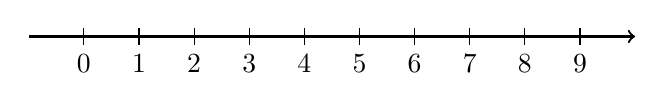
\begin{tikzpicture}[scale=0.7]
  \draw[thick,->] (-1,0) -- (10,0);
  \foreach \x in {0,...,9} \draw (\x,0.15) -- (\x,-0.15) node[below] {$\x$};
\end{tikzpicture}
\end{center}
\end{questionText}
\correctAnswer{$x \geq 4$; closed circle at $4$, shade right}
\explanation{Add $4$: $3x \geq 12$. Divide by $3$: $x \geq 4$. Closed circle at $4$, shade right.}
\end{practiceQuestion}

\begin{practiceQuestion}{5-6-q26}{gsa}
\begin{questionText}
Solve $-2x + 5 > 11$ and graph the solution.

\begin{center}
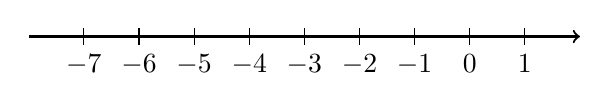
\begin{tikzpicture}[scale=0.7]
  \draw[thick,->] (-8,0) -- (2,0);
  \foreach \x in {-7,...,1} \draw (\x,0.15) -- (\x,-0.15) node[below] {$\x$};
\end{tikzpicture}
\end{center}
\end{questionText}
\correctAnswer{$x < -3$; open circle at $-3$, shade left}
\explanation{Subtract $5$: $-2x > 6$. Divide by $-2$ and flip: $x < -3$. Open circle at $-3$, shade left.}
\end{practiceQuestion}

\begin{practiceQuestion}{5-6-q27}{gsa}
\begin{questionText}
A student scored at least $75$ on every test. The number line below shows the possible scores $s$. Write the inequality and state whether $75$ is included.

\begin{center}
\begin{tikzpicture}[scale=0.06]
  \draw[thick,->] (600,0) -- (1050,0);
  \foreach \x in {65,70,...,100} {
    \pgfmathsetmacro\pos{\x*10}
    \draw (\pos,2) -- (\pos,-2) node[below] {$\x$};
  }
  \draw[thick,funBlue,->] (750,0) -- (1050,0);
  \fill[funBlue] (750,0) circle (60pt);
\end{tikzpicture}
\end{center}
\end{questionText}
\correctAnswer{$s \geq 75$; yes, $75$ is included}
\explanation{The closed circle at $75$ means $75$ is included. Shading to the right means all scores $75$ and above: $s \geq 75$.}
\end{practiceQuestion}
